% Created by tikzDevice version 0.10.1 on 2018-01-12 15:55:52
% !TEX encoding = UTF-8 Unicode
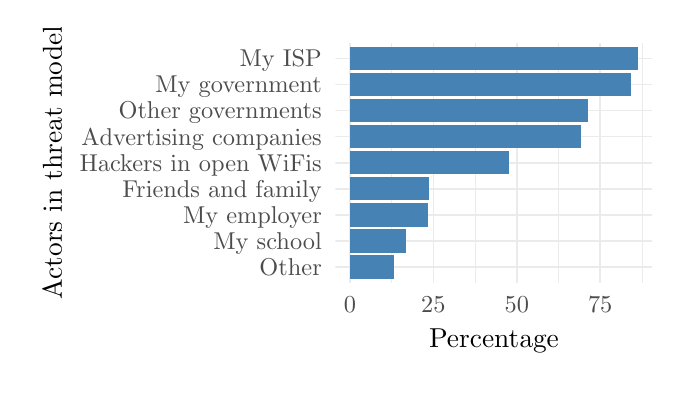
\begin{tikzpicture}[x=1pt,y=1pt]
\definecolor{fillColor}{RGB}{255,255,255}
\path[use as bounding box,fill=fillColor,fill opacity=0.00] (0,0) rectangle (231.26,122.86);
\begin{scope}
\path[clip] (111.23, 30.77) rectangle (225.76,117.36);
\definecolor{drawColor}{gray}{0.92}

\path[draw=drawColor,line width= 0.3pt,line join=round] (131.51, 30.77) --
	(131.51,117.36);

\path[draw=drawColor,line width= 0.3pt,line join=round] (161.66, 30.77) --
	(161.66,117.36);

\path[draw=drawColor,line width= 0.3pt,line join=round] (191.81, 30.77) --
	(191.81,117.36);

\path[draw=drawColor,line width= 0.3pt,line join=round] (221.96, 30.77) --
	(221.96,117.36);

\path[draw=drawColor,line width= 0.6pt,line join=round] (111.23, 36.42) --
	(225.76, 36.42);

\path[draw=drawColor,line width= 0.6pt,line join=round] (111.23, 45.83) --
	(225.76, 45.83);

\path[draw=drawColor,line width= 0.6pt,line join=round] (111.23, 55.24) --
	(225.76, 55.24);

\path[draw=drawColor,line width= 0.6pt,line join=round] (111.23, 64.65) --
	(225.76, 64.65);

\path[draw=drawColor,line width= 0.6pt,line join=round] (111.23, 74.07) --
	(225.76, 74.07);

\path[draw=drawColor,line width= 0.6pt,line join=round] (111.23, 83.48) --
	(225.76, 83.48);

\path[draw=drawColor,line width= 0.6pt,line join=round] (111.23, 92.89) --
	(225.76, 92.89);

\path[draw=drawColor,line width= 0.6pt,line join=round] (111.23,102.30) --
	(225.76,102.30);

\path[draw=drawColor,line width= 0.6pt,line join=round] (111.23,111.71) --
	(225.76,111.71);

\path[draw=drawColor,line width= 0.6pt,line join=round] (116.44, 30.77) --
	(116.44,117.36);

\path[draw=drawColor,line width= 0.6pt,line join=round] (146.59, 30.77) --
	(146.59,117.36);

\path[draw=drawColor,line width= 0.6pt,line join=round] (176.73, 30.77) --
	(176.73,117.36);

\path[draw=drawColor,line width= 0.6pt,line join=round] (206.88, 30.77) --
	(206.88,117.36);
\definecolor{fillColor}{RGB}{70,130,180}

\path[fill=fillColor] (116.44, 32.18) rectangle (132.22, 40.66);

\path[fill=fillColor] (116.44, 41.60) rectangle (136.81, 50.07);

\path[fill=fillColor] (116.44, 51.01) rectangle (144.81, 59.48);

\path[fill=fillColor] (116.44, 60.42) rectangle (145.04, 68.89);

\path[fill=fillColor] (116.44, 69.83) rectangle (173.88, 78.30);

\path[fill=fillColor] (116.44, 79.24) rectangle (199.96, 87.71);

\path[fill=fillColor] (116.44, 88.65) rectangle (202.48, 97.12);

\path[fill=fillColor] (116.44, 98.07) rectangle (218.04,106.54);

\path[fill=fillColor] (116.44,107.48) rectangle (220.56,115.95);
\end{scope}
\begin{scope}
\path[clip] (  0.00,  0.00) rectangle (231.26,122.86);
\definecolor{drawColor}{gray}{0.30}

\node[text=drawColor,anchor=base east,inner sep=0pt, outer sep=0pt, scale=  0.88] at (106.28, 33.39) {Other};

\node[text=drawColor,anchor=base east,inner sep=0pt, outer sep=0pt, scale=  0.88] at (106.28, 42.80) {My school};

\node[text=drawColor,anchor=base east,inner sep=0pt, outer sep=0pt, scale=  0.88] at (106.28, 52.21) {My employer};

\node[text=drawColor,anchor=base east,inner sep=0pt, outer sep=0pt, scale=  0.88] at (106.28, 61.62) {Friends and family};

\node[text=drawColor,anchor=base east,inner sep=0pt, outer sep=0pt, scale=  0.88] at (106.28, 71.04) {Hackers in open WiFis};

\node[text=drawColor,anchor=base east,inner sep=0pt, outer sep=0pt, scale=  0.88] at (106.28, 80.45) {Advertising companies};

\node[text=drawColor,anchor=base east,inner sep=0pt, outer sep=0pt, scale=  0.88] at (106.28, 89.86) {Other governments};

\node[text=drawColor,anchor=base east,inner sep=0pt, outer sep=0pt, scale=  0.88] at (106.28, 99.27) {My government};

\node[text=drawColor,anchor=base east,inner sep=0pt, outer sep=0pt, scale=  0.88] at (106.28,108.68) {My ISP};
\end{scope}
\begin{scope}
\path[clip] (  0.00,  0.00) rectangle (231.26,122.86);
\definecolor{drawColor}{gray}{0.30}

\node[text=drawColor,anchor=base,inner sep=0pt, outer sep=0pt, scale=  0.88] at (116.44, 19.76) {0};

\node[text=drawColor,anchor=base,inner sep=0pt, outer sep=0pt, scale=  0.88] at (146.59, 19.76) {25};

\node[text=drawColor,anchor=base,inner sep=0pt, outer sep=0pt, scale=  0.88] at (176.73, 19.76) {50};

\node[text=drawColor,anchor=base,inner sep=0pt, outer sep=0pt, scale=  0.88] at (206.88, 19.76) {75};
\end{scope}
\begin{scope}
\path[clip] (  0.00,  0.00) rectangle (231.26,122.86);
\definecolor{drawColor}{RGB}{0,0,0}

\node[text=drawColor,anchor=base,inner sep=0pt, outer sep=0pt, scale=  0.99] at (168.50,  7.44) {Percentage};
\end{scope}
\begin{scope}
\path[clip] (  0.00,  0.00) rectangle (231.26,122.86);
\definecolor{drawColor}{RGB}{0,0,0}

\node[text=drawColor,rotate= 90.00,anchor=base,inner sep=0pt, outer sep=0pt, scale=  0.99] at ( 12.32, 74.07) {Actors in threat model};
\end{scope}
\end{tikzpicture}
